\begin{abstract}
	As privacy protection mechanisms are not necessarily visible to the user it is hard to demonstrate their effectiveness.
	We present several visualizations, which can be used for that purpose.
\end{abstract}

% ------------------------------------------------------------------------------
\section{Introduction}
Privacy protection mechanisms have to be integrated into applications, frameworks, and services.
Many of these mechanisms work without the user noticing anything.
When such mechanisms are in effect in the background, a demonstration of their effectiveness might prove difficult.

In this paper we present different visualizaitons that can be used to demonstrate the effectiveness of privacy protection mechanisms for document storage services.
Document storage services can be used by multiple users in order to store their documents or files.
Documents are usually tied to a user's account and are identified uniquely per user by their name and path.
Lots of personal information can be inferred from data stored in such a service.
Operators can abuse this information or it can unintentionally get leaked.
Privacy protection mechanisms can be integrated to protect personal information.

However, demonstrating the effectiveness of such mechanisms by showing the contents of the database or log entries of the service is hard to comprehend.
We therefore present several visualizations with the aim to make the effect of some protection mechanism more comprehensible.

\begin{figure*}[ht]
	\centering
	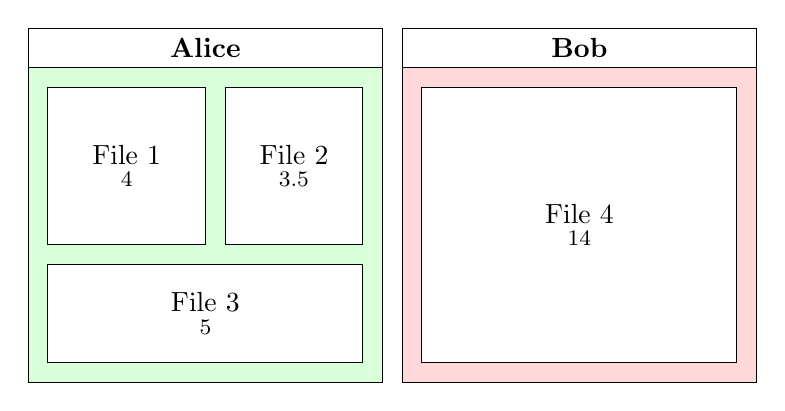
\begin{tikzpicture}
	% Alice
	\draw (.25,4.25) rectangle ++(4.5,.5) node[pos=.5] {\textbf{Alice}};
	\draw[fill=green!15] (.25,.25) rectangle ++(4.5,4);
	\draw[fill=white] (.5,2) rectangle ++(2,2) node[pos=.5] {%
		\shortstack{%
			File 1\\
			\footnotesize\SI{4}{\mebi\byte}
		}
	};
	\draw[fill=white] (2.75,2) rectangle ++(1.75,2) node[pos=.5] {%
		\shortstack{%
			File 2\\
			\footnotesize\SI{3.5}{\mebi\byte}
		}
	};
	\draw[fill=white] (.5,.5) rectangle ++(4,1.25) node[pos=.5] {%
		\shortstack{%
			File 3\\
			\footnotesize\SI{5}{\mebi\byte}
		}
	};

	% Bob
	\draw (5,4.25) rectangle ++(4.5,.5) node[pos=.5] {\textbf{Bob}};
	\draw[fill=red!15] (5,.25) rectangle ++(4.5,4);
	\draw[fill=white] (5.25,.5) rectangle ++(4,3.5) node[pos=.5] {%
		\shortstack{%
			File 4\\
			\footnotesize\SI{14}{\mebi\byte}
		}
	};
\end{tikzpicture}

	\caption{Visualizaton of files of different sizes belonging to two user accounts.}%
	\label{fig:metadata-treemap}
\end{figure*}

\begin{figure*}[ht]
	\centering
	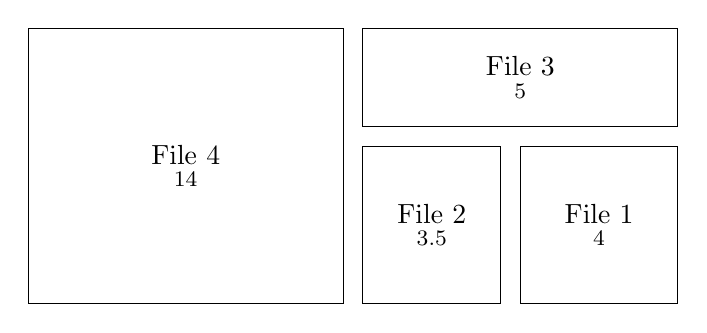
\begin{tikzpicture}
	%\draw (0,0) rectangle ++(8.75,4);
	\draw (.25,.25) rectangle ++(4,3.5) node[pos=.5] {%
		\shortstack{%
			File 4\\
			\footnotesize\SI{14}{\mebi\byte}
		}
	};
	\draw (4.5,.25) rectangle ++(1.75,2) node[pos=.5] {%
		\shortstack{%
			File 2\\
			\footnotesize\SI{3.5}{\mebi\byte}
		}
	};
	\draw (6.5,.25) rectangle ++(2,2) node[pos=.5] {%
		\shortstack{%
			File 1\\
			\footnotesize\SI{4}{\mebi\byte}
		}
	};
	\draw (4.5,2.5) rectangle ++(4,1.25) node[pos=.5] {%
		\shortstack{%
			File 3\\
			\footnotesize\SI{5}{\mebi\byte}
		}
	};
\end{tikzpicture}


	\caption{Visualizaton of files of different sizes, where the file's owner is not known.}%
	\label{fig:filesonly-treemap}
\end{figure*}

% ------------------------------------------------------------------------------
\section{Setting}
In order to be able to demonstrate the effectiveness of such protection mechanisms we have developed a document storage, which can imitate a malicious service operator.
This is done by collecting as much information as possible, including traffic data like IP addresses, geolocation of networks, and metadata like file sizes.
The history of each document is preserved, so that even if a client issues a request to delete the document to the service, the serivce operator will still be able to access the file afterwards.
He reports to the client, that the file has been removed, so from the client's perspective the service functions normally.
The document storage is offered as a web service, which can be accessed using a REST-style API.
Each HTTP request will be logged completely.

As the service including the visualizations or introspection APIs might be publicly accessible on the Internet, this behavior would violate privacy regulations of most countries.
Therefore, the malicious behavior of the service is only enabled if the client opts in by setting the \mintinline{http}{X-AppPETs-BadProvider: 1} HTTP header.
Additional HTTP headers are used to determine ground truth, e.\,g., if the identity of the client is protected by a specific mechanism, the identity can be provided additionally.
This allows to evaluate the accuracy of heuristical inference attacks.

The visualizations are offered as web pages by the service and supports animations as well as interactions.

% ------------------------------------------------------------------------------

\begin{figure*}[t]
	\centering
	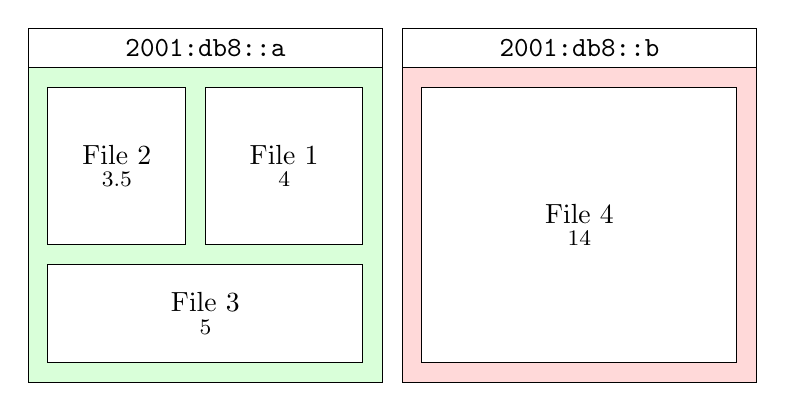
\begin{tikzpicture}
	% Alice
	\draw (0,4.25) rectangle ++(4.5,.5) node[pos=.5] {\textbf{\texttt{2001:db8::a}}};
	\draw[fill=green!15] (0,.25) rectangle ++(4.5,4);
	\draw[fill=white] (.25,2) rectangle ++(1.75,2) node[pos=.5] {%
		\shortstack{%
			File 2\\
			\footnotesize\SI{3.5}{\mebi\byte}
		}
	};
	\draw[fill=white] (2.25,2) rectangle ++(2,2) node[pos=.5] {%
		\shortstack{%
			File 1\\
			\footnotesize\SI{4}{\mebi\byte}
		}
	};
	\draw[fill=white] (.25,.5) rectangle ++(4,1.25) node[pos=.5] {%
		\shortstack{%
			File 3\\
			\footnotesize\SI{5}{\mebi\byte}
		}
	};

	% Bob
	\draw (4.75,4.25) rectangle ++(4.5,.5) node[pos=.5] {\textbf{\texttt{2001:db8::b}}};
	\draw[fill=red!15] (4.75,.25) rectangle ++(4.5,4);
	\draw[fill=white] (5,.5) rectangle ++(4,3.5) node[pos=.5] {%
		\shortstack{%
			File 4\\
			\footnotesize\SI{14}{\mebi\byte}
		}
	};
\end{tikzpicture}

	\caption{Visualizaton of files of different sizes, grouped by the sender's IP address.}%
	\label{fig:ip-treemap}
\end{figure*}

\begin{figure*}[t]
	\centering
	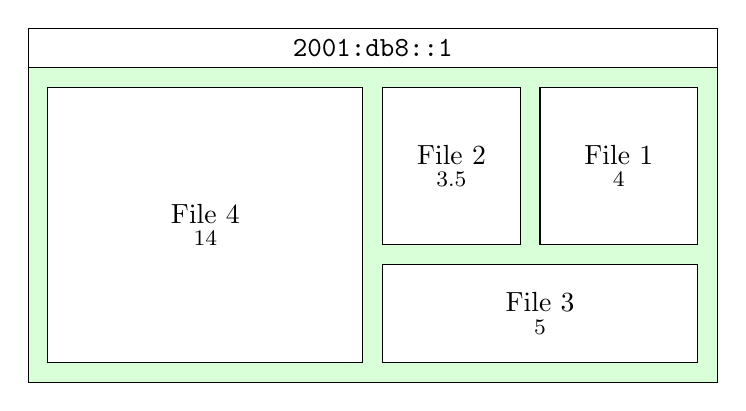
\begin{tikzpicture}
	\draw (.25,4.25) rectangle ++(8.75,.5) node[pos=.5] {\textbf{\texttt{2001:db8::1}}};
	\draw[fill=green!15] (.25,.25) rectangle ++(8.75,4);
	\draw[fill=white] (.5,.5) rectangle ++(4,3.5) node[pos=.5] {%
		\shortstack{%
			File 4\\
			\footnotesize\SI{14}{\mebi\byte}
		}
	};
	\draw[fill=white] (4.75,2) rectangle ++(1.75,2) node[pos=.5] {%
		\shortstack{%
			File 2\\
			\footnotesize\SI{3.5}{\mebi\byte}
		}
	};
	\draw[fill=white] (6.75,2) rectangle ++(2,2) node[pos=.5] {%
		\shortstack{%
			File 1\\
			\footnotesize\SI{4}{\mebi\byte}
		}
	};
	\draw[fill=white] (4.75,.5) rectangle ++(4,1.25) node[pos=.5] {%
		\shortstack{%
			File 3\\
			\footnotesize\SI{5}{\mebi\byte}
		}
	};
\end{tikzpicture}

	\caption{Visualizaton of files of different sizes, grouped by the sender's IP address. All senders use the same proxy server.}%
	\label{fig:proxy-treemap}
\end{figure*}

\begin{figure*}[t]
	\centering
	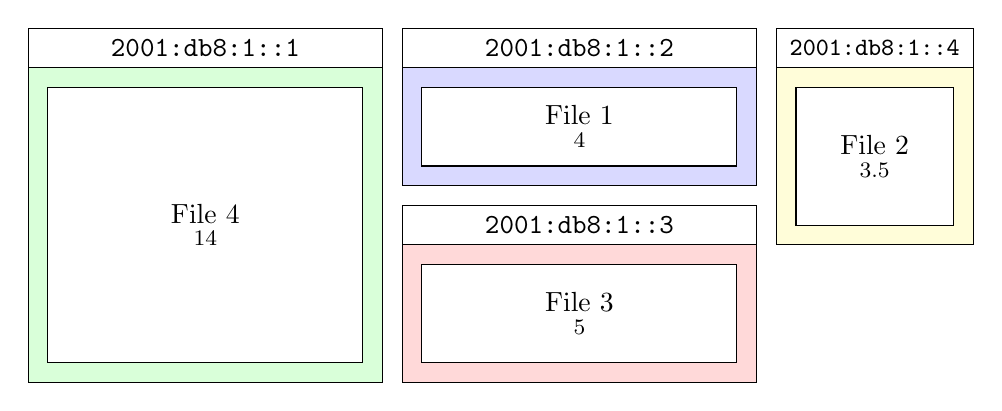
\begin{tikzpicture}
	\draw (0,4) rectangle ++(4.5,.5) node[pos=.5] {\textbf{\texttt{2001:db8:1::1}}};
	\draw[fill=green!15] (0,0) rectangle ++(4.5,4);
	\draw[fill=white] (.25,.25) rectangle ++(4,3.5) node[pos=.5] {%
		\shortstack{%
			File 4\\
			\footnotesize\SI{14}{\mebi\byte}
		}
	};

	\draw (4.75,4) rectangle ++(4.5,.5) node[pos=.5] {\textbf{\texttt{2001:db8:1::2}}};
	\draw[fill=blue!15] (4.75,2.5) rectangle ++(4.5,1.5);
	\draw[fill=white] (5,2.75) rectangle ++(4,1) node[pos=.5] {%
		\shortstack{%
			File 1\\
			\footnotesize\SI{4}{\mebi\byte}
		}
	};

	\draw (4.75,1.75) rectangle ++(4.5,.5) node[pos=.5] {\textbf{\texttt{2001:db8:1::3}}};
	\draw[fill=red!15] (4.75,0) rectangle ++(4.5,1.75);
	\draw[fill=white] (5,.25) rectangle ++(4,1.25) node[pos=.5] {%
		\shortstack{%
			File 3\\
			\footnotesize\SI{5}{\mebi\byte}
		}
	};

	\draw (9.5,4) rectangle ++(2.5,.5) node[pos=.5] {\small\textbf{\texttt{2001:db8:1::4}}};
	\draw[fill=yellow!15] (9.5,1.75) rectangle ++(2.5,2.25);
	\draw[fill=white] (9.75,2) rectangle ++(2,1.75) node[pos=.5] {%
		\shortstack{%
			File 2\\
			\footnotesize\SI{3.5}{\mebi\byte}
		}
	};
\end{tikzpicture}

	\caption{Visualizaton of files of different sizes, grouped by the sender's IP address. The senders use an anonymization service that uses a different IP address for each request.}%
	\label{fig:acn-treemap}
\end{figure*}

\section{Scenarios}
We discuss some selected scenarios and present mock-ups for possible visualizations.

\subsection{Content and Metadata}
A document storage without privacy protection mechanisms stores the files as they are.
They are tied to the account of the file owner.

The state of the document storage service can be visualized as a tree map~\cite{DBLP:journals/ivs/GrahamK10}.
The files are rectangular leaf nodes and their size is derived from the file's size.
Files are grouped by the user account of their owner, as depicted in~\cref{fig:metadata-treemap}.
Additional metadata will be displayed when clicking on a file node, such as a preview of the content as well as a link to download the original file.
Metadata of files could be used for further visualizations, in order to demonstrate what a service operator can learn about its users if they have access to the files contents.
Possible visualizations with differing effects on the data subjects (file owners) are presented by \textcite{DBLP:journals/popets/HarkousRKA16,Krause:2017}.

\subsection{Traffic Data}
We further assume that content and metadata are protected in a way, that the service provider can not link them to specific user accounts, e.\,g., as presented by \textcite{securekeyvaluestorage-whitepaper}.
The file sizes and file identifiers will be kept, so that differences can be spotted.
The same previous visualization method can then not group files per user account anymore, as depicted in~\cref{fig:filesonly-treemap}.

We assume that the client communicates directly with the service.
A malicious service operator can now link the files by the client's IP address, e.\,g., if Alice has the IP address \texttt{2001:db8::a} and Bob has the IP address \texttt{2001:db8::b}, the grouping can be restored as depicted in~\cref{fig:ip-treemap}.
Note that the server might not know which IP address belongs to Alice or to Bob.
The address can still be used to deduce which files belong to the same user.

The IP addresses can also be used to see where Alice and Bob where located when they modified or retrieved files.
As depicted in~\cref{fig:geolocation}, Alice interacted with a file 1 in Hamburg, then moved to Berlin and interacted with files 2 and 3.
Bob is located in Nuremberg.
A similar visualization based on EXIF metadata of photos has been proposed by \textcite{Krause:2017}.

\begin{figure}[h]
	\centering
	\begin{tikzpicture}
	\node[anchor=south west,inner sep=0] at (0,0) {%
		\includegraphics[width=.95\columnwidth]{figures/germany}
	};

	%\draw[help lines,xstep=1,ystep=1] (0,0) grid (8,11);

	\node[draw,thick,fill=green!15] (f1) at (3.5,8) {File 1};
	\node[draw,thick,fill=green!15] (f2) at (6,6.5) {File 2 \& 3};

	\draw[-{Latex[length=3mm]},thick] (f1) -- (f2);

	\node[draw,thick,fill=red!15] at (4.5,2.5) {File 4};
\end{tikzpicture}

	\caption[A map showing the locations where files were uploaded.]{A map\footnotemark\ showing the locations where files were uploaded.}%
	\label{fig:geolocation}
\end{figure}
\footnotetext{Map taken from \url{https://pixelmap.amcharts.com}}

We want to protect the client's IP addresses as well and use two different methods for this purpose to highlight their differences from the service's perspective.
First, the same proxy server with the IP address \texttt{2001:db8::1} is used for all clients, e.\,g., as presented by \textcite{DBLP:conf/icccn/PanchenkoWPA09}.
All users are in the same anonymity group.
The service operator now only sees a single sender IP address, as depicted in~\cref{fig:proxy-treemap}, which is quite similar to~\cref{fig:filesonly-treemap}.
Second, an anonymous communication network is used, e.\,g., Tor or JAP.
It is used in a way, that each request is sent through a different IP address with the prefix \texttt{2001:db8:1}.
The information derived as depicted in~\cref{fig:acn-treemap} cannot be used to reliably link files to either Alice or Bob.

The problem is not solved however, as different methods can be used to link multiple requests to the same user.
Proxies usually attach additional traffic data that allows linkage, as presented by \textcite{DBLP:journals/corr/PerinoSV16}.
\textcite{DBLP:conf/pet/Eckersley10} present fingerprinting techniques based on HTTP headers, and \textcite{DBLP:journals/ejisec/HusakCJC16} present such techniques for TLS connections.

% ------------------------------------------------------------------------------
\section{Demonstrator}
An open source key-value storage service has been implemented in Python, which can be used to store documents\footnote{AppPETs/PrivacyService: Implementation of privacy-friendly services: \url{https://github.com/AppPETs/PrivacyService}}.
Visualizations have been implemented with \textit{D3.js} JavaScript library and are accessible through the service directly.
Not all the proposed visualizations have been implemented as described at the time of writing.
In addition to visualizations an introspection API was added that can be used to retrieve the data collected by the service.
This can be used to realize visualizations on the user's device.

% ------------------------------------------------------------------------------
\section{Conclusion}
Several visualizations have been proposed and a demo service was developed which implement some of these visualizations.
A user study should be performed in order to validate that the visualizations are helpful in understanding effects of privacy protection mechanisms on document storage services.

Additional information could be collected from the client as well, which would allow creating even more helpful visualizations of data processing and data protection mechanisms.
One example of visualizing data flows for an application was proposed by \textcite{DBLP:conf/nordsec/Kani-ZabihiH11}.

The visualizations presented in this paper as well as visualizations from related work could also be used for interactive privacy policies as they might be able to explain complex data processing and protection mechanisms in a comprehensive manner.
